\documentclass{article}

\usepackage{indentfirst}
\usepackage[utf8]{inputenc}
\usepackage[margin = 1.5cm]{geometry}
\usepackage{graphicx}
\usepackage{float}

\usepackage{hyperref} % Insert hyperlinks
\hypersetup{
colorlinks = true,
linkcolor = blue,
urlcolor = blue,
citecolor = black}
\usepackage{url} % Insert URLs
\usepackage{comment} % In-line comments

\usepackage{natbib} % Citation formatting

\title{Report on Data Gathering for MESSAGEix Canada}
\author{Noah Leverton}
\date{December 2021}

\begin{document}

\maketitle

\tableofcontents

\newpage

% \begin{itemize}
%     \item Project goals/MESSAGEix details
%     \begin{itemize}
%         \item Create a provinicial Canadian model based off of the national model
%         \item Downscale input variables
%         \item Account for the different industries, demographics of the provinces of Canada
%     \end{itemize}
%     \item Sources (info found in ppt)
%     \begin{itemize}
%         \item Open Gov
%         \item Natural Resources Can
%         \item Statistics Canada
%         \item Energy Future (Canada Energy Regulator)
%     \end{itemize}
%     \item Data Categories
%     \item Methods
%     \begin{itemize}
%         \item My background going into the project (minimal)
%         \item Excel
%         \item Python packages
%         \begin{itemize}
%             \item pandas
%             \item pyam
%         \end{itemize}
%     \end{itemize}
%     \item Downscaling
%     \begin{itemize}
%         \item Mostly used pyam function
%         \item Description of how the function works
%         \item Weaknesses of this crude method
%     \end{itemize}
%     \item Documentation for continuing work on MESSAGEix
    
% \end{itemize}

\section{Intro (Project goals/MESSAGEix details)}

The main focus of this project was to develop a provincial-scale version of the MESSAGEix Canada model. MESSAGEix is an integrated assessment model for climate change with global coverage \citep{messageDocs}. A Canadian version of the model was developed by Muhammad Awais, who oversaw the development of the provincial model this term. As Canada's energy system is made up of varying policies and technologies across the provinces, it was necessary to account for this by developing a provincial model. As well, population density varies considerably by province, and as population and GDP data are central inputs to IAMs, an accurate representation of the provinces was vital to providing a more accurate picture of the Canadian energy system. 

My role in the project was to gather data for several inputs to the MESSAGEix model, clean/format that data, and downscale any variables which either could not be found or could only be found at a national scale. As my experience with data analysis was limited (arguably non-existent), the process was initially slow. 

\section{Sources}

My main sources of data for this project were Statistics Canada (\citeyear{statCan}), Canada Energy Regulator \citep{CER}, Natural Resources Canada (\citeyear{nrcan}) and Open Government Canada (\citeyear{openGov}).

\subsection{Statistics Canada}

Statistics Canada was a useful source due to the level of control it offers for output data. In the case of the energy supply and demand table which I sourced data from, the data could be filtered by province, sector, fuel, etc. This was useful as it meant I had less processing/filtering to do later on. Statistics Canada data can also be exported in multiple formats, including one csv format for database loading which was especially useful.

This source is not without it's drawbacks though. There were ranges of years for some data which were missing, as well as data which was reported for some provinces but not others. As I needed data for every province, these data gaps meant Statistics Canada was a much less useful source than I had initially thought it would be. Some of the data from this source also had empty entries where there should have been zero-values. This initially seemed an easy problem to remedy but due to the fact that it was difficult to discern which cells should be filled with zeros, and which should be marked as 'unreported data' it ended up being a roadblock to my progress.

\subsection{Canada Energy Regulator}

Canada Energy Regulator was a useful source as it has projections to 2050 for several end-use energy demands (MESSAGEix needs end-use energy demand projections to 2060 as input). This ended up being invaluable for the aggregated categories, but less useful for the more specific data I needed. CER does however offer some more specific data for the transportation sector. The main drawback of this source was the lack of specificity. The multiple scenarios of it's end-use demand projections could prove useful, as they could allow for multiple runs of the MESSAGEix provincial model based off of different (Federal) policy assumptions.

\subsection{Natural Resources Canada}

Natural Resources Canada is useful for the level of specificity it offers, mainly for energy use in the residential and commercial sectors. NRCAN has over a decade's worth of data for space heating/cooling energy usage, which MESSAGEix needs as input. This source did prove to be laborious to export from however, as one must navigate to a different webpage for each sector and province and download individual spreadsheets of data. While this likely could have been simplified with some html coding, this was beyond my level of expertise and as the amount of data I needed from NRCAN was not too great, I was able to export it manually. The format of the data exported from NRCAN was also more geared towards human readability than something that could be read into python, meaning some amount of manual cleaning had to be performed.

\subsection{Open Government Canada}

Open Government Canada data was used minimally (mainly for import/export data). The format of the data was easy to read into python, but offered little control (over file-type of output, filtering, etc.).

\section{Data Categories}

Data was gathered for many different categories, some (but not all) of which are listed below.
% Could change this to a two column list to save space

\begin{itemize}
    \item End-use demand
    \begin{itemize}
        \item Residential + Commercial Specific\footnote{Requires electricity \citep{messageDocs}}/Thermal\footnote{Does not require electricity \citep{messageDocs}}
        \item Industrial Specific/Thermal/Feedstocks
        \item Transportation
    \end{itemize}
    \item Electrical generation and capacity
    \begin{itemize}
        \item Biomass
        \item Coal
        \item Heavy fuel oil
        \item Light fuel oil (diesel, gasoline)
        \item Natural gas (combined cylinder and combustion turbine)
        \item Hydro
        \item Nuclear
        \item Solar PV
        \item Wind
    \end{itemize}
    \item Imports/Exports
    \begin{itemize}
        \item Coal
        \item Crude oil
        \item Electricity
        \item Ethanol
        \item Heavy/light fuel oil
        \item Natural gas
    \end{itemize}
    \item Production
    \begin{itemize}
        \item Coal extraction
        \item Gas extraction
        \item Energy transmission/distribution
    \end{itemize}
\end{itemize}

I started by gathering data for the end-use categories at the top. Initially the data sets were relatively small, and I mainly used Excel for manual editing. As I moved to the more specific categories further down the list, my methods had to be changed for the sake of consistency and efficiency.

\newpage

\section{Methods}

\subsection{Excel}

I went into this project with very minimal experience using Excel, and learned that while it is useful for quick and dirty data processing, it leaves plenty of room for human error. Manual editing can also be laborious, and though I do not doubt Excel can be a powerful and efficient tool in the hands of an expert, I am far from an expert. Nevertheless I feel much more capable working with excel for simple operations now that my co-op has concluded (including moving and renaming subsets of data, simple mathematical and string operations). 

\subsection*{pandas}

pandas is a package for python which is mainly used for analyzing and performing bulk operations on data. It was very useful for quickly finding gaps in data (empty cells in a spreadsheet), as well as verifying the validity of data (looking for outliers, maintaining consistent units). The learning process for pandas was quite slow, and operations that would have been trivial in Excel proved much less so with pandas. As most of the data processing I was performing was fairly simple I only used the basic features of pandas, but I enjoyed the learning process and feel much better equipped to take on data analysis tasks in the future.

\subsection{pyam}

pyam is another python package, used for similar data analysis tasks as pandas but specifically designed for use with IAMs. pyam also offers plenty of options for filtering and plotting data, which was useful when I needed plots of the data I had gathered for my presentation to the SESIT group. It offers a good middle ground between excel and pandas, as it is built off the latter and has functions to perform operations that are less intuitive when using pandas alone (adding data rows together, renaming cells in bulk, etc.).

pyam is also useful for unit conversion due to it's interface with the \href{https://pint.readthedocs.io/en/stable/}{pint package}. This was invaluable as most MESSAGEix parameters were needed in gigawatts, and most of the data gathered was reported in joules. While pandas can convert units using multiple operations, pyam has an intuitive function for completing this task in one step.

\section{Downscaling}

In cases where a data point either could not be found, or was only found at a national scale, downscaling had to be employed. While this process can be accomplished in multiple ways, it basically boils down to using mathematical or statistical methods to translate aggregated data to dis-aggregated, specific data. I mainly used a pyam function for downscaling, which employs a simple (if crude) method of regional downscaling, illustrated in figure \ref{downscalingFigure}.
\begin{figure}[H]
    \centering
    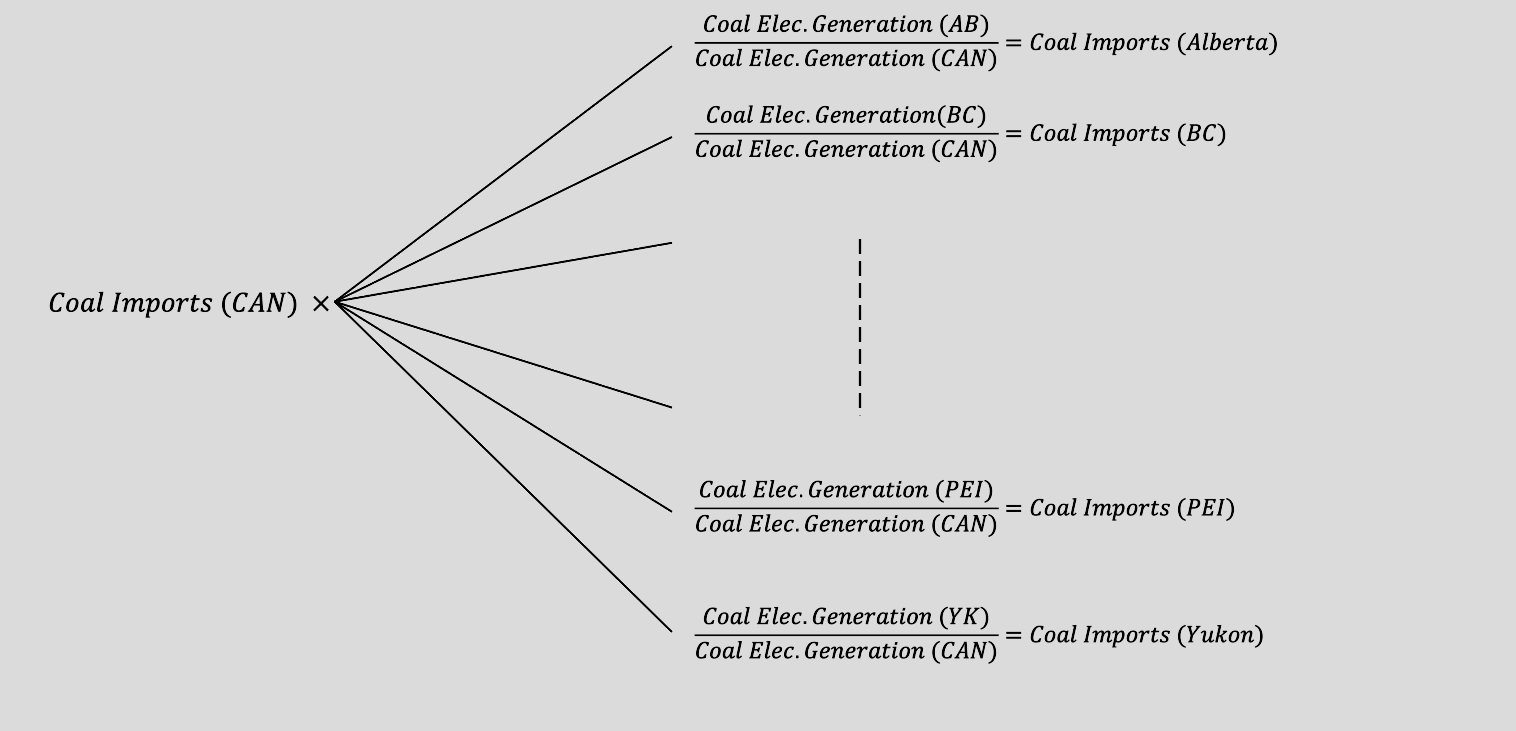
\includegraphics[width=0.8\textwidth]{figures/downscalingFigure.png}
    \caption{Downscaling Example}
    \label{downscalingFigure}
\end{figure}
In this example, suppose we only have national data for coal imports, but we have provincial data for electricity generation from coal. We take the weights of coal electricity generation (our proxy variable) for each province by dividing the provincial value by the national one, and then multiply this weight by the national value for coal imports to get a provincial value for coal imports. This has the obvious effect of homogenizing the data and creating many identical trajectories, which makes sense in some cases but necessitates choosing an appropriate proxy variable. Also, care must be taken to avoid misrepresenting the provinces: in cases where numerical data cannot be found, some amount of research should be done to decide which provinces to include in the weighting. For example, even if we do not have numerical data for a province, we may know from our research that the province has access to coal locally and so does not import at all, in which case we would omit it from our weighting and instead distribute among the remaining provinces.

\section{Documentation for continuing work on MESSAGEix}

As my co-op term drew to a close I was tasked with completing some basic documentation to get a future co-op student up to speed on the MESSAGEix model and the data gathering process. This documentation was added to the GitLab repository for the model (see the README.md files in the repository).

% The following is meant to get a future co-op student up to speed on the provincial MESSAGEix model, and lists all necessary skills to ensure a smooth transition. The section title have links to relevant documentation when applicable. My number one advice is to stay organized. Make sure you have consistent naming for any excel sheets containing data, organize your data in the repository in a logical way, and keep a record of all of your sources somewhere (I wasn't good at this initially which lead to headaches later in the project).

% \subsection*{\href{https://docs.messageix.org/en/stable/}{MESSAGEix}}

% Information on installing MESSAGEix on your machine can be found \href{https://docs.messageix.org/en/stable/install.html}{here}. Main things to know include:

% \begin{itemize}
%     \item How to create a scenario, add parameters to it
%     \item The format of MESSAGEix parameter dataframes (the make\_df function handles this)
%     \item How to read in parameters from the national model
%     \item What the parameter names mean in MESSAGEix (\href{https://docs.messageix.org/projects/models/en/stable/pkg-data/codelists.html}{this} is a good reference)
% \end{itemize}

% \subsection*{Python/Programming Stuff}

% If you have taken an introductory coding course you should be fine, specific things which are important for this project include:

% \begin{itemize}
%     \item pandas/pyam packages
%     \item matplotlib
%     \item anaconda: creating environments and installing packages
%     \item knowledge of a python IDE (this is mostly personal preference, although I found jupyter notebooks (or jupyter lab) useful as it displays dataframes inline and in a more legible way than other IDEs)
% \end{itemize}

% \subsection*{Excel}

% My experience with Excel was minimal going into this project, an engineering student would probably be much more proficient. A co-op student should be able to convert data from one format to another (I often had to convert from wide to long date format) using excel (or pandas if they know how to use it). 

% \subsection*{\href{https://git-scm.com/book/en/v2/Git-Basics-Getting-a-Git-Repository}{git}}

% I had zero experience with git at the start of my co-op, but the basics are quick to learn and that was really all I needed. Make sure you know how to:

% \begin{itemize}
%     \item Clone a repository, and update the main repository using the commit and push commands
%     \item Create an ssh key to grant authentication to update the MESSAGEix repository
%     \item Create a branch of a repository
%     \item Create a .gitignore file (although there are templates of these which you can copy at \url{https://github.com/github/gitignore})
% \end{itemize}

% \subsection*{\href{https://pandas.pydata.org/pandas-docs/stable/getting_started/index.html\#getting-started}{pandas}}

% This package is slow to learn at first but is much more efficient than Excel in the long run and has less room for human error. Make sure you know:

% \begin{itemize}
%     \item The basics of pandas' two data structures (series and dataframes)
%     \item How to read .csv and .xlsx files with pandas
%     \item The various methods of filtering and indexing dataframes (\url{https://pandas.pydata.org/pandas-docs/stable/user_guide/indexing.html})
% \end{itemize}

% \subsection*{\href{https://pyam-iamc.readthedocs.io/en/stable/index.html}{pyam}}

% If learning how to use pandas proves too much of a hassle initially, pyam is a good package which simplifies some of it's operations. Make sure you know:

% \begin{itemize}
%     \item The format of pyam dataframes (these are specifically designed to organize data from IAMs)
%     \item Filtering in pyam
%     \item pyam's downscaling function
% \end{itemize}

% \subsection*{Data sources}

% All relevant sources for the data gathered so far for MESSAGEix are found in the gitlab repository (data/provincial\_sources).

\newpage

\bibliography{reportBibliography}
\bibliographystyle{apalike}

\end{document}
